\begin{figure}[ht!]
	\centering
	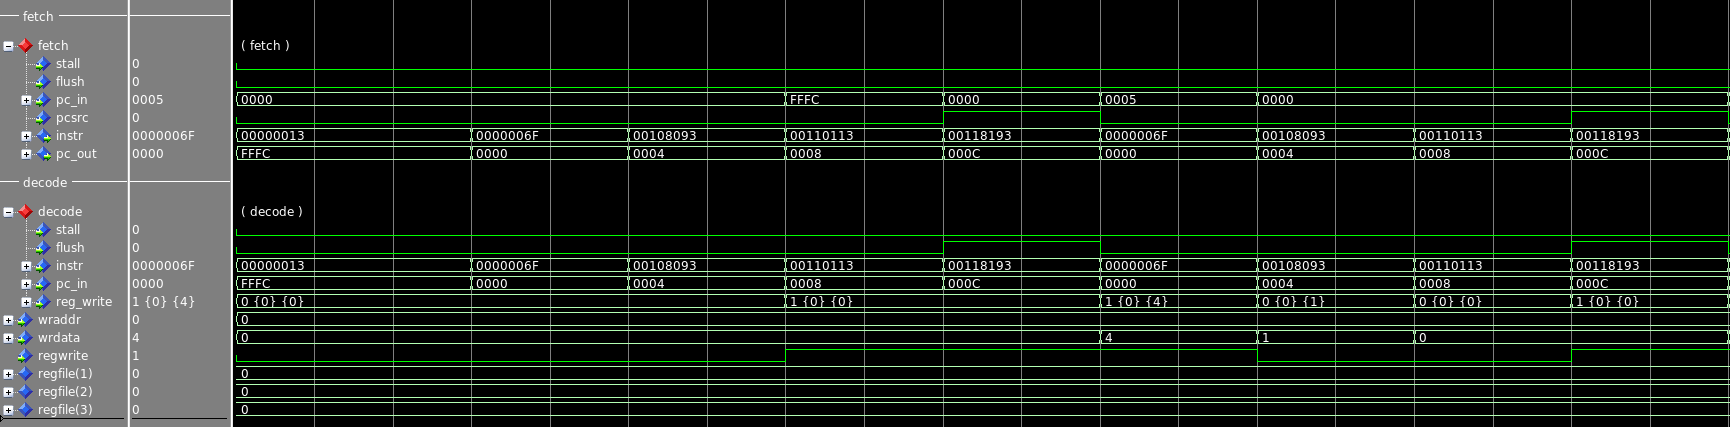
\includegraphics[width=1.0\linewidth]{ctrl.png}
	\caption{Simulation screenshot for Listing~\ref{lst:asmbds}.}
	\label{fig:sim2}
\end{figure}

Make sure that at least the following signals are visible in
Figure~\ref{fig:sim2}: the program counter in the fetch stage, the
instruction being fetched, the content of registers \texttt{x1}, 
\texttt{x2} and \texttt{x3} as well as the signals \texttt{wraddr},
\texttt{wrdata} and \texttt{regwrite} of the register file.

\begin{lstlisting}[language=,mathescape=false,float=ht,caption={Assembler example for branches},label=lst:asmbds]
loop:   j loop
        addi x1, x1, 1
        addi x2, x2, 1
        addi x3, x3, 1
\end{lstlisting}

